% Options for packages loaded elsewhere
\PassOptionsToPackage{unicode}{hyperref}
\PassOptionsToPackage{hyphens}{url}
\PassOptionsToPackage{dvipsnames,svgnames,x11names}{xcolor}
%
\documentclass[
  singlecolumn]{report}

\usepackage{amsmath,amssymb}
\usepackage{iftex}
\ifPDFTeX
  \usepackage[T1]{fontenc}
  \usepackage[utf8]{inputenc}
  \usepackage{textcomp} % provide euro and other symbols
\else % if luatex or xetex
  \usepackage{unicode-math}
  \defaultfontfeatures{Scale=MatchLowercase}
  \defaultfontfeatures[\rmfamily]{Ligatures=TeX,Scale=1}
\fi
\usepackage[]{libertinus}
\ifPDFTeX\else  
    % xetex/luatex font selection
\fi
% Use upquote if available, for straight quotes in verbatim environments
\IfFileExists{upquote.sty}{\usepackage{upquote}}{}
\IfFileExists{microtype.sty}{% use microtype if available
  \usepackage[]{microtype}
  \UseMicrotypeSet[protrusion]{basicmath} % disable protrusion for tt fonts
}{}
\makeatletter
\@ifundefined{KOMAClassName}{% if non-KOMA class
  \IfFileExists{parskip.sty}{%
    \usepackage{parskip}
  }{% else
    \setlength{\parindent}{0pt}
    \setlength{\parskip}{6pt plus 2pt minus 1pt}}
}{% if KOMA class
  \KOMAoptions{parskip=half}}
\makeatother
\usepackage{xcolor}
\usepackage[top=30mm,left=20mm,heightrounded]{geometry}
\setlength{\emergencystretch}{3em} % prevent overfull lines
\setcounter{secnumdepth}{-\maxdimen} % remove section numbering
% Make \paragraph and \subparagraph free-standing
\ifx\paragraph\undefined\else
  \let\oldparagraph\paragraph
  \renewcommand{\paragraph}[1]{\oldparagraph{#1}\mbox{}}
\fi
\ifx\subparagraph\undefined\else
  \let\oldsubparagraph\subparagraph
  \renewcommand{\subparagraph}[1]{\oldsubparagraph{#1}\mbox{}}
\fi


\providecommand{\tightlist}{%
  \setlength{\itemsep}{0pt}\setlength{\parskip}{0pt}}\usepackage{longtable,booktabs,array}
\usepackage{calc} % for calculating minipage widths
% Correct order of tables after \paragraph or \subparagraph
\usepackage{etoolbox}
\makeatletter
\patchcmd\longtable{\par}{\if@noskipsec\mbox{}\fi\par}{}{}
\makeatother
% Allow footnotes in longtable head/foot
\IfFileExists{footnotehyper.sty}{\usepackage{footnotehyper}}{\usepackage{footnote}}
\makesavenoteenv{longtable}
\usepackage{graphicx}
\makeatletter
\def\maxwidth{\ifdim\Gin@nat@width>\linewidth\linewidth\else\Gin@nat@width\fi}
\def\maxheight{\ifdim\Gin@nat@height>\textheight\textheight\else\Gin@nat@height\fi}
\makeatother
% Scale images if necessary, so that they will not overflow the page
% margins by default, and it is still possible to overwrite the defaults
% using explicit options in \includegraphics[width, height, ...]{}
\setkeys{Gin}{width=\maxwidth,height=\maxheight,keepaspectratio}
% Set default figure placement to htbp
\makeatletter
\def\fps@figure{htbp}
\makeatother
\newlength{\cslhangindent}
\setlength{\cslhangindent}{1.5em}
\newlength{\csllabelwidth}
\setlength{\csllabelwidth}{3em}
\newlength{\cslentryspacingunit} % times entry-spacing
\setlength{\cslentryspacingunit}{\parskip}
\newenvironment{CSLReferences}[2] % #1 hanging-ident, #2 entry spacing
 {% don't indent paragraphs
  \setlength{\parindent}{0pt}
  % turn on hanging indent if param 1 is 1
  \ifodd #1
  \let\oldpar\par
  \def\par{\hangindent=\cslhangindent\oldpar}
  \fi
  % set entry spacing
  \setlength{\parskip}{#2\cslentryspacingunit}
 }%
 {}
\usepackage{calc}
\newcommand{\CSLBlock}[1]{#1\hfill\break}
\newcommand{\CSLLeftMargin}[1]{\parbox[t]{\csllabelwidth}{#1}}
\newcommand{\CSLRightInline}[1]{\parbox[t]{\linewidth - \csllabelwidth}{#1}\break}
\newcommand{\CSLIndent}[1]{\hspace{\cslhangindent}#1}

\usepackage{booktabs}
\usepackage{longtable}
\usepackage{array}
\usepackage{multirow}
\usepackage{wrapfig}
\usepackage{float}
\usepackage{colortbl}
\usepackage{pdflscape}
\usepackage{tabu}
\usepackage{threeparttable}
\usepackage{threeparttablex}
\usepackage[normalem]{ulem}
\usepackage{makecell}
\usepackage{xcolor}
\usepackage{cancel}
\makeatletter
\makeatother
\makeatletter
\makeatother
\makeatletter
\@ifpackageloaded{caption}{}{\usepackage{caption}}
\AtBeginDocument{%
\ifdefined\contentsname
  \renewcommand*\contentsname{Table of contents}
\else
  \newcommand\contentsname{Table of contents}
\fi
\ifdefined\listfigurename
  \renewcommand*\listfigurename{List of Figures}
\else
  \newcommand\listfigurename{List of Figures}
\fi
\ifdefined\listtablename
  \renewcommand*\listtablename{List of Tables}
\else
  \newcommand\listtablename{List of Tables}
\fi
\ifdefined\figurename
  \renewcommand*\figurename{Figure}
\else
  \newcommand\figurename{Figure}
\fi
\ifdefined\tablename
  \renewcommand*\tablename{Table}
\else
  \newcommand\tablename{Table}
\fi
}
\@ifpackageloaded{float}{}{\usepackage{float}}
\floatstyle{ruled}
\@ifundefined{c@chapter}{\newfloat{codelisting}{h}{lop}}{\newfloat{codelisting}{h}{lop}[chapter]}
\floatname{codelisting}{Listing}
\newcommand*\listoflistings{\listof{codelisting}{List of Listings}}
\makeatother
\makeatletter
\@ifpackageloaded{caption}{}{\usepackage{caption}}
\@ifpackageloaded{subcaption}{}{\usepackage{subcaption}}
\makeatother
\makeatletter
\@ifpackageloaded{tcolorbox}{}{\usepackage[skins,breakable]{tcolorbox}}
\makeatother
\makeatletter
\@ifundefined{shadecolor}{\definecolor{shadecolor}{rgb}{.97, .97, .97}}
\makeatother
\makeatletter
\makeatother
\makeatletter
\makeatother
\ifLuaTeX
  \usepackage{selnolig}  % disable illegal ligatures
\fi
\IfFileExists{bookmark.sty}{\usepackage{bookmark}}{\usepackage{hyperref}}
\IfFileExists{xurl.sty}{\usepackage{xurl}}{} % add URL line breaks if available
\urlstyle{same} % disable monospaced font for URLs
\hypersetup{
  pdftitle={Better causal diagrammes (DAGS) for counterfactual data science},
  pdfauthor={Joseph A. Bulbulia},
  colorlinks=true,
  linkcolor={blue},
  filecolor={Maroon},
  citecolor={Blue},
  urlcolor={Blue},
  pdfcreator={LaTeX via pandoc}}

\title{Better causal diagrammes (DAGS) for counterfactual data science}
\author{Joseph A. Bulbulia}
\date{}

\begin{document}
\maketitle
\ifdefined\Shaded\renewenvironment{Shaded}{\begin{tcolorbox}[boxrule=0pt, frame hidden, borderline west={3pt}{0pt}{shadecolor}, interior hidden, sharp corners, breakable, enhanced]}{\end{tcolorbox}}\fi

\listoffigures
\listoftables
\hypertarget{abstract}{%
\section{Abstract}\label{abstract}}

\hypertarget{introduction}{%
\section{Introduction}\label{introduction}}

\[A \coprod Y(a)$ and $A \cancel{\coprod} Y(a)| L\]

\hypertarget{objective}{%
\subsection{Objective}\label{objective}}

Correlation is not causation. However, across many human sciences,
persistent confusion in the analysis and reporting of correlations has
limited scientific progress. The correlations in observed data are
frequently biased indicators of causality. This problem is widely known.
Nevertheless, many researchers report correlations using hedging
language that may suggest causation. Widespread practices of reporting
correlations -- in which I have regrettably participated -- has led to a
``causality crisis'' (\protect\hyperlink{ref-bulbulia2022}{Bulbulia
2022}). The problem is a crisis, because we cannot generally estimate
causal effects from observational data. Widely adopted strategies for
``control'' fail. Addressing the causality crisis is arguably among
science's most pressing issues.

When integrated into methodologically rigorous workflows, causal
diagrammes or causal directed acyclic graphs -- causal ``DAGs'' -- may
be powerful tools for identifying causation.\footnote{The term ``DAG''
  is unfortunate because not all directed acyclic graphs are causal. For
  a graph to be causal it must satisfy the conditions of markov
  factorisation (see Appendix A). In my utopia, I would preferred that
  causal diagrammes were called markov factorisation graphs (see
  Appendix A).} Yet unscrupulous DAGs operate in much the same way as
hedging correlational language, suggesting entitlement to causal
inferences where none are warrented. For example, when researchers lack
time-series data they cannot generally estimate unbiased causal
effects(\protect\hyperlink{ref-vanderweele2015}{VanderWeele 2015}).
Thus, cross-sectional researchers who use DAGs to report the unrealistic
assumptions embedded in their analyses use the tool to disguise
unwarrented confidence. Ideally causal diagrammes would be equipped with
safety mechanisms that prevent such self-inflicted injuries.

Here, I develop a guide to writing causal diagrammes that is grounding
in temporally ordered representations of their key elements -- what
might be called \emph{chronologically conscientious} causal DAGs. We
shall see that attention to temporal order in the spatial organisation
of a DAG may greatly assist researchers in avoiding the pitfalls of
unscrupulous DAGs. Although no inferential tool is user-proof, the
application of chronologically conscientious DAGs may improve saftey.
Chronologically conscientious causal diagrammes are DAGs with airbags.

There are many excellent resources for drawing causal diagrammes
(\protect\hyperlink{ref-rohrer2018}{Rohrer 2018};
\protect\hyperlink{ref-hernan2023}{Hernan and Robins 2023};
\protect\hyperlink{ref-cinelli2022}{Cinelli, Forney, and Pearl 2022};
\protect\hyperlink{ref-barrett2021}{Barrett 2021};
\protect\hyperlink{ref-mcelreath2020}{McElreath 2020}).\footnote{In my
  view, currently the best resource is Miguel Hernan's free course,
  here:
  \url{https://pll.harvard.edu/course/causal-diagrams-draw-your-assumptions-your-conclusions}.}
One may reasonably question whether another tutorial merely adds
clutter. The approach to drawing causal diagrammes that I present hopes
to contributes to previous attempts in five ways. First, I link graphs
to the counterfactual frameworks that are necessary for conceptualising
causality. Second, as mentioned, I underscore the importance of
chronology in the presentation of the graph. Along the way, I use causal
graphs to examine the concepts of interaction and mediation, again with
the aim of guiding applied researchers clear of trouble. Third, I show
how causal diagrammes to recommend a three-wave panel design for
recording cultural evolutionary dynamics in the present. Fourth, I
consider the problem of selection bias three-wave panel designs, and
develop recommendations for applied researchers. Fifth, I consider the
problem of measurement bias in three-wave panel designs, and develop
recommendations for applied researchers. I conclude with a brief
compendium of practical advice to help researchers avoid abominable DAGs
and causal inferences.

The article is organised as follows:

\textbf{Part 1.} develops the connection between causal diagrammes and
the potential outcomes framework. Understanding this connection is
important. Whereas causal diagrammes help researchers to answer
questions, we must first understand how to ask causal questions. Without
such comprehension, causal graphs can be, at best, unproductive, and at
worst, deceptive.

\textbf{Part 2.} reviews the four elemental types of confounding, and
uses chronologically conscientious causal diagrammes to elucidate their
properties. Although this discussion replicates material from other
tutorials, by emphasising the temporal order in spatial structure of the
graph the conditions in which we may identify causality in the presence
of confounding become more apparent. Here, I show how causal graphs may
clarify concepts of interaction, mediation, and treatment-confounder
feedback of the kind we may expect to be pervasive time-series data.
Finally, I describe a simple template that may be useful for
evolutionary human scientists, which clarifies how three-waves of data
collection may be used to estimate causal effects.

\textbf{Part 3.} Applies chronologically conscientious causal diagrammes
to motivate three-wave panel designs for evolutionary social sciences

\textbf{Part 4} Addresses substanative problems of selection bias,
focussing attention on the imperatives for adequate sampling and
retention in the three-wave panel design.

\textbf{Part 5.} Addresses substanative problems of measurement error,
focussing attention on the imperatives of (a) ensuring good measures (b)
assessing pathways for confounding (c) performing sensitivity analyses.

Technical details are presented in an Appendix.

\hypertarget{part-1.-identifiability-assumptions}{%
\section{Part 1. Identifiability
assumptions}\label{part-1.-identifiability-assumptions}}

Causal diagrammes are powerful tools for answering causal questions.
However before we can answer a causal question, we must first understand
what is involved when we ask a causal question. In this section I review
key concepts and identification assumptions.

\hypertarget{the-fundamental-problem-of-causal-inference}{%
\subsection{The fundamental problem of causal
inference}\label{the-fundamental-problem-of-causal-inference}}

We say that \(A\) causes \(Y\) if changing \(A\) would have made a
difference to the outcome of \(Y\). The use of the subjective ``would
have'' reveals the need for counterfactuals when conceiving of causal
effects. To infere a causal effect requires \emph{counterfactual
data-science}.

Suppose there is evidence that cultures believing in Big Gods
demonstrate greater social complexity. We are interested in estimating
the causal effect of belief in Big Gods on social complexity. Here, the
belief in Big Gods is the ``exposure'' or ``treatment'' of interest.

We define two counterfactual (or ``potential'') outcomes for each
culture in a population:

\begin{itemize}
\tightlist
\item
  \(Y_i(a = 1)\): The social complexity of culture \(i\) if they
  believed in Big Gods. This is the counterfactual outcome when
  \(A_i = 1\).
\item
  \(Y_i(a = 0)\): The social complexity of culture \(i\) if they did not
  believe in Big Gods. This is the counterfactual outcome when
  \(A_i = 0\).
\end{itemize}

Within a counterfactual framework, the causal effect of belief in Big
Gods on social complexity for culture \(i\) may be defined as a
contrast, on the difference scale, between two potential outcomes
(\(Y_i(a)\)) under the two different levels of the exposure (\(A_i = 1\)
(belief in Big Gods); \(A_i = 0\) (no belief in Big Gods)). For
simplicity we assume these exposures are exhaustive, and well-defined.
Under these assumptions:

\[
\text{Causal Effect of Belief in Big Gods}_i = Y_i(1) - Y_i(0) 
\]

We require a contrast between two states of the world only one of which
the culture might actually receive \footnote{The counter-factual outcome
  under the exposure \(A = a\) may be written in different ways, such as
  \(Y(a)\) (the notation we use here), \(Y^a\), and \(Y_a\).}. When the
culture receives one level of the belief in Big Gods the outcome under
the other level(s) is ruled out by the natural order. The same holds for
groups of cultures who are exposed or unexposed. This is called ``the
fundamental problem of causal inference''
(\protect\hyperlink{ref-rubin1976}{Rubin 1976};
\protect\hyperlink{ref-holland1986}{Holland 1986}). As shown in
Table~\ref{tbl-consistency}, at least half the counterfactual outcomes
we require for estimating individual causal effects are missing. For
this reason, causal inference has been described as a missing data
problem (\protect\hyperlink{ref-westreich2015}{Westreich et al. 2015};
\protect\hyperlink{ref-edwards2015}{Edwards, Cole, and Westreich 2015}).

Table~\ref{tbl-consistency} expresses the relationship between
observable and counterfactual outcomes as a contingency table (This
table is modified from a table in
(\protect\hyperlink{ref-morgan2014}{Morgan and Winship 2014})).

\hypertarget{tbl-consistency}{}
\begin{longtable}[]{@{}
  >{\raggedright\arraybackslash}p{(\columnwidth - 4\tabcolsep) * \real{0.0779}}
  >{\raggedright\arraybackslash}p{(\columnwidth - 4\tabcolsep) * \real{0.4416}}
  >{\raggedright\arraybackslash}p{(\columnwidth - 4\tabcolsep) * \real{0.4805}}@{}}
\caption{\label{tbl-consistency}Causal estimation as a missing data
problem.}\tabularnewline
\toprule\noalign{}
\begin{minipage}[b]{\linewidth}\raggedright
Group
\end{minipage} & \begin{minipage}[b]{\linewidth}\raggedright
Units that receive exposure (A=1)
\end{minipage} & \begin{minipage}[b]{\linewidth}\raggedright
Units that recieve no exposure (A=0)
\end{minipage} \\
\midrule\noalign{}
\endfirsthead
\toprule\noalign{}
\begin{minipage}[b]{\linewidth}\raggedright
Group
\end{minipage} & \begin{minipage}[b]{\linewidth}\raggedright
Units that receive exposure (A=1)
\end{minipage} & \begin{minipage}[b]{\linewidth}\raggedright
Units that recieve no exposure (A=0)
\end{minipage} \\
\midrule\noalign{}
\endhead
\bottomrule\noalign{}
\endlastfoot
Y(1) & Observable & Counterfactual \\
Y(0) & Counterfactual & Observable \\
\end{longtable}

\begin{figure}

{\centering 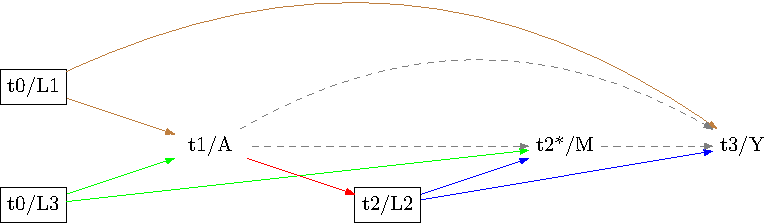
\includegraphics[width=0.8\textwidth,height=\textheight]{test-again_files/figure-pdf/fig-dag-mediation-assuptions-1.pdf}

}

\caption{\label{fig-dag-mediation-assuptions}Assumptions for mediation
analysis}

\end{figure}

\hypertarget{refs}{}
\begin{CSLReferences}{1}{0}
\leavevmode\vadjust pre{\hypertarget{ref-barrett2021}{}}%
Barrett, Malcolm. 2021. \emph{Ggdag: Analyze and Create Elegant Directed
Acyclic Graphs}. \url{https://CRAN.R-project.org/package=ggdag}.

\leavevmode\vadjust pre{\hypertarget{ref-bulbulia2022}{}}%
Bulbulia, Joseph A. 2022. {``A Workflow for Causal Inference in
Cross-Cultural Psychology.''} \emph{Religion, Brain \& Behavior} 0 (0):
1--16. \url{https://doi.org/10.1080/2153599X.2022.2070245}.

\leavevmode\vadjust pre{\hypertarget{ref-cinelli2022}{}}%
Cinelli, Carlos, Andrew Forney, and Judea Pearl. 2022. {``A Crash Course
in Good and Bad Controls.''} \emph{Sociological Methods \& Research},
May, 00491241221099552. \url{https://doi.org/10.1177/00491241221099552}.

\leavevmode\vadjust pre{\hypertarget{ref-edwards2015}{}}%
Edwards, Jessie K, Stephen R Cole, and Daniel Westreich. 2015. {``All
Your Data Are Always Missing: Incorporating Bias Due to Measurement
Error into the Potential Outcomes Framework.''} \emph{International
Journal of Epidemiology} 44 (4): 14521459.

\leavevmode\vadjust pre{\hypertarget{ref-hernan2023}{}}%
Hernan, M. A., and J. M. Robins. 2023. \emph{Causal Inference}. Chapman
\& Hall/CRC Monographs on Statistics \& Applied Probab. Taylor \&
Francis. \url{https://books.google.co.nz/books?id=/_KnHIAAACAAJ}.

\leavevmode\vadjust pre{\hypertarget{ref-holland1986}{}}%
Holland, Paul W. 1986. {``Statistics and Causal Inference.''}
\emph{Journal of the American Statistical Association} 81 (396): 945960.

\leavevmode\vadjust pre{\hypertarget{ref-mcelreath2020}{}}%
McElreath, Richard. 2020. \emph{Statistical Rethinking: A Bayesian
Course with Examples in r and Stan}. CRC press.

\leavevmode\vadjust pre{\hypertarget{ref-morgan2014}{}}%
Morgan, Stephen L., and Christopher Winship. 2014. \emph{Counterfactuals
and Causal Inference: Methods and Principles for Social Research}. 2nd
ed. Analytical Methods for Social Research. Cambridge: Cambridge
University Press. \url{https://doi.org/10.1017/CBO9781107587991}.

\leavevmode\vadjust pre{\hypertarget{ref-rohrer2018}{}}%
Rohrer, Julia M. 2018. {``Thinking Clearly about Correlations and
Causation: Graphical Causal Models for Observational Data.''}
\emph{Advances in Methods and Practices in Psychological Science} 1 (1):
2742.

\leavevmode\vadjust pre{\hypertarget{ref-rubin1976}{}}%
Rubin, D. B. 1976. {``Inference and Missing Data.''} \emph{Biometrika}
63 (3): 581--92. \url{https://doi.org/10.1093/biomet/63.3.581}.

\leavevmode\vadjust pre{\hypertarget{ref-vanderweele2015}{}}%
VanderWeele, Tyler. 2015. \emph{Explanation in Causal Inference: Methods
for Mediation and Interaction}. Oxford University Press.

\leavevmode\vadjust pre{\hypertarget{ref-westreich2015}{}}%
Westreich, Daniel, Jessie K Edwards, Stephen R Cole, Robert W Platt,
Sunni L Mumford, and Enrique F Schisterman. 2015. {``Imputation
Approaches for Potential Outcomes in Causal Inference.''}
\emph{International Journal of Epidemiology} 44 (5): 17311737.

\end{CSLReferences}



\end{document}
